\usetikzlibrary{arrows.meta,calc}

\begin{frame}[fragile]{flood-to-search}
\begin{tikzpicture}
\tikzset{
    nd/.style={draw,circle,very thick,font=\fontsize{7}{8}\selectfont,alt=<4-5>{opacity=0.2}},
    query mark/.style={blue,line width=0.8mm,-Latex,dotted,alt=<4-5>{opacity=0.2}},
    query/.style={draw,blue,solid,font=\fontsize{8}{9}\selectfont\tt,inner sep=0.3mm,thick,align=left,alt=<4-5>{opacity=0.2}},
    reject/.style={violet},
    hilite/.style={opacity=1},
}
\node[nd] (A) at (0, 0) {A};
\node[nd] (B) at (2, 5) {B};
\node[nd] (C) at (3, -2){C};
\node[nd] (D) at (2, 2) {D};
\node[nd,alt=<4>{hilite,fill=red!10}] (E) at (4, 0){E};
\node[nd] (F) at (6, 2) {F};
\node[nd] (G) at (6, 4) {G};
\node[nd,alt=<5>{hilite,fill=red!10}] (H) at (4, 5) {H};
\foreach \x/\y in {A/B,A/C,B/D,D/E,E/F,C/E,F/G,G/H} {
    \draw[very thick,Latex-Latex] (\x) -- (\y);
}

\begin{visibleenv}<2-5>
    \draw[query mark] (A) -- (B)
        node[midway,above left,query] {
            Query: `foo'\\  TTL=3 \\
            ID = ab312\ldots fe
        };
    \draw[query mark] (A) -- (C)
        node[midway,below left,query] {
            Query: `foo'\\ TTL=3 \\
            ID = ab312\ldots fe
        };
    \draw[query mark] (B) -- (D)
        node[midway,right,query] {
            Query: `foo'\\ TTL=2 \\
            ID = ab312\ldots fe
        };
    \draw[query mark,reject,alt=<4>{hilite}] (D) -- (E)
        node[midway,below left,query,violet,alt=<4>{hilite}] {
            Query: `foo'\\ TTL=1 \\
            ID = ab312\ldots fe
        };
    \draw[query mark,alt=<4>{hilite}] (C) -- (E)
        node[midway,below right,query,alt=<4>{hilite}] {
            Query: `foo'\\ TTL=2 \\
            ID = ab312\ldots fe
        };
    \draw[query mark] (E) -- (F) 
        node[midway,below right,query] {
            Query: `foo'\\ TTL=2 \\
            ID = ab312\ldots fe
        };
    \draw[query mark] (F) -- (G) 
        node[midway,left,query] {
            Query: `foo'\\ TTL=1 \\
            ID = ab312\ldots fe
        };
\end{visibleenv}
\begin{visibleenv}<6>
    \draw[query mark] (D) -- (B)
        node[midway,right,query] {
            Query Response: \\
            file \ldots at 1.2.3.4 \\
            ID = ab321\ldots fe
        };
    \draw[query mark] (B) -- (A)
        node[midway,right,query] {
            Query Response: \\
            file \ldots at 1.2.3.4 \\
            ID = ab321\ldots fe
        };
\end{visibleenv}
\coordinate (explain loc) at (7, 5);
\coordinate (explain loc low) at (6, 0);
\tikzset{
    explain box gen/.style={align=left,anchor=north west},
    explain box/.style={align=left,at={(explain loc)},anchor=north west},
    explain box low/.style={align=left,at={(explain loc low)},anchor=north west},
}
\begin{visibleenv}<3>
\node[explain box] {
    every node forwards \\
    to neighbors  \\
    (similar to link-state \\
    routing flooding)
};
\end{visibleenv}
\begin{visibleenv}<4>
\node[explain box low] {
    nodes reject duplicates \\
    using query ID
};
\end{visibleenv}
\begin{visibleenv}<5>
\node[explain box gen,anchor=south west,overlay] at ([xshift=1cm]H) {
    if TTL not high enough \\
    query won't get to all nodes
};
\end{visibleenv}
\begin{visibleenv}<6>
\node[explain box] {
    nodes with response(s) \\
    send back 
};
\end{visibleenv}
\end{tikzpicture}
\end{frame}

\begin{frame}{small worlds}
    \begin{itemize}
    \item might seem we need high TTL, so queries slow\ldots
    \item but not really:
        \begin{itemize}
        \item typical nodes have 10s of peers, not 1 or 2
        \item rouhgly random connections make it likely paths are short
        \end{itemize}
    \item some figures from paper by Stutzbach, Rajaie, and Sen in 2005
    \end{itemize}
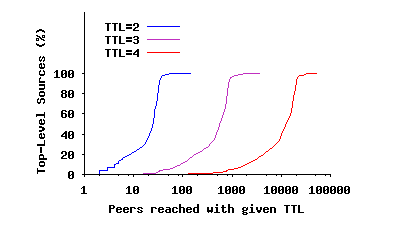
\includegraphics[width=0.4\textwidth]{../p2p/stutzbach-fig6b} 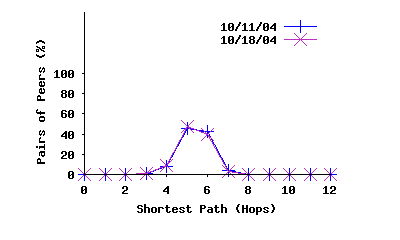
\includegraphics[width=0.4\textwidth]{../p2p/stutzbach-fig7b}
\imagecredit{Stutzbach, et al. ``Characterizing Unstructured Overlay Topologies in Modern P2P File-Sharing Systems'' (IMC'05)}
\end{frame}

\begin{frame}{not scaling}
    \begin{itemize}
    \item flood-to-search pretty inefficient with large network
    \vspace{.5cm}
    \item Gnutella did some optimizations that undecentralize network some:
        \begin{itemize}
        \item split nodes into ultrapeers and leafs
        \item ultrapeers copy whole index for nearby leafs
        \end{itemize}
    \end{itemize}
\end{frame}
